\paragraph{}
En esta sección se especificará con detalle cada una de las pantallas que
componen \juego. Además, se indicarán las transiciones entre ellas así
como la utilidad de cada elemento de la GUI (\emph{Graphical User Interface}).
Las imágenes adjuntas son bocetos que ilustran los componentes que debe contener
cada pantalla, no obstante, los artistas podrán (y deberán) hacer cambios en la apariencia
y disposición de los elementos si así lo consideran oportuno.


\subsection{Diagrama de flujo}
\label{sec:ui-flujo}

\paragraph{}
El siguiente diagrama de estados muestra las pantallas presentes a lo largo
de \juego y las transiciones entre ellas. En puntos posteriores nos centraremos
en ellas de forma individual.

\begin{figure}[H]
    \centering
        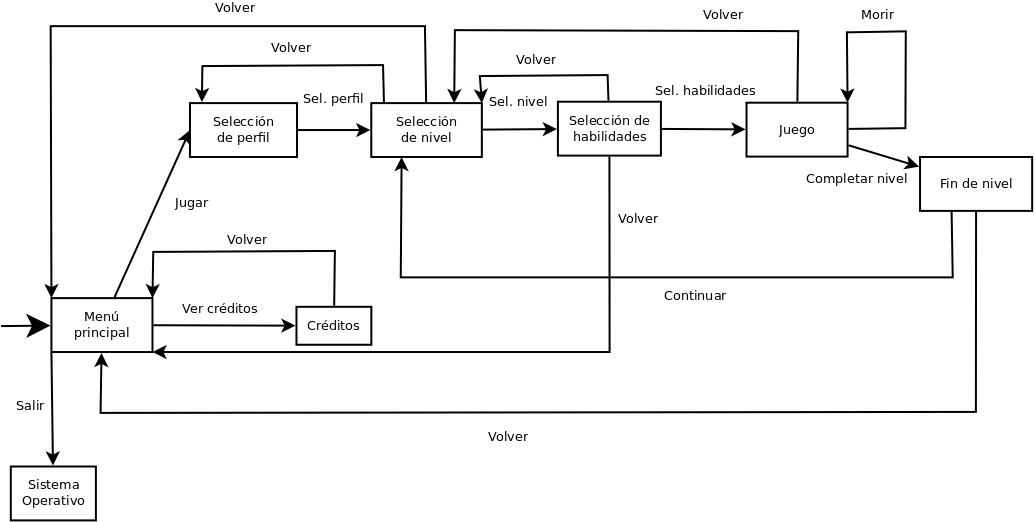
\includegraphics[width=\textwidth]{img/flowchart.png} 
    \caption{Diagrama de flujo de pantallas en el juego}
    \label{img:flowchart}
\end{figure}

\clearpage

\subsection{Menú principal}
\label{sec:ui-menu}

\paragraph{}
A continuación el boceto de la pantalla de \menu:

\begin{figure}[H]
    \centering
        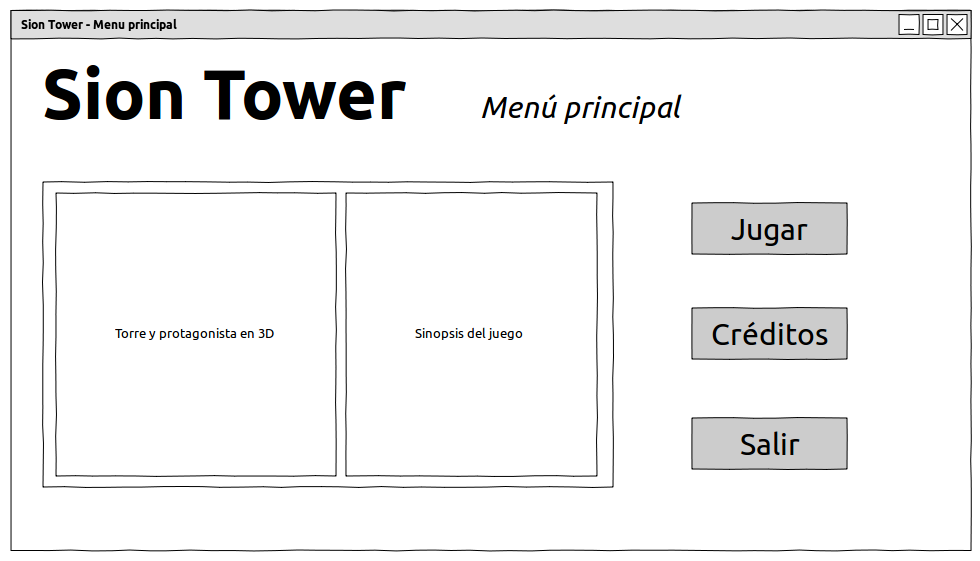
\includegraphics[width=\textwidth]{img/menu-principal.png} 
    \caption{Boceto del menú principal}
    \label{img:menu-principal}
\end{figure}

\paragraph{}
Lista y descripción de todos sus componentes.

\begin{itemize}
    \item \textbf{Botón jugar}: al pulsarlo lleva a la pantalla \selperfil.
    \item \textbf{Botón créditos}: al pulsarlo lleva a la pantalla \creditos.
    \item \textbf{Botón salir}: al pulsarlo nos lleva de vuelta al Sistema Operativo.
    \item \textbf{Torre y protagonista}: vista 3D de la torre (\juego) y del
    protagonista a modo de ambientación.
    \item \textbf{Sinopsis}: texto con una breve introducción a la historia
    del juego.
\end{itemize}

\clearpage

\subsection{Créditos}
\label{sec:ui-creditos}

\paragraph{}
A continuación el boceto de la pantalla de \creditos:

\begin{figure}[H]
    \centering
        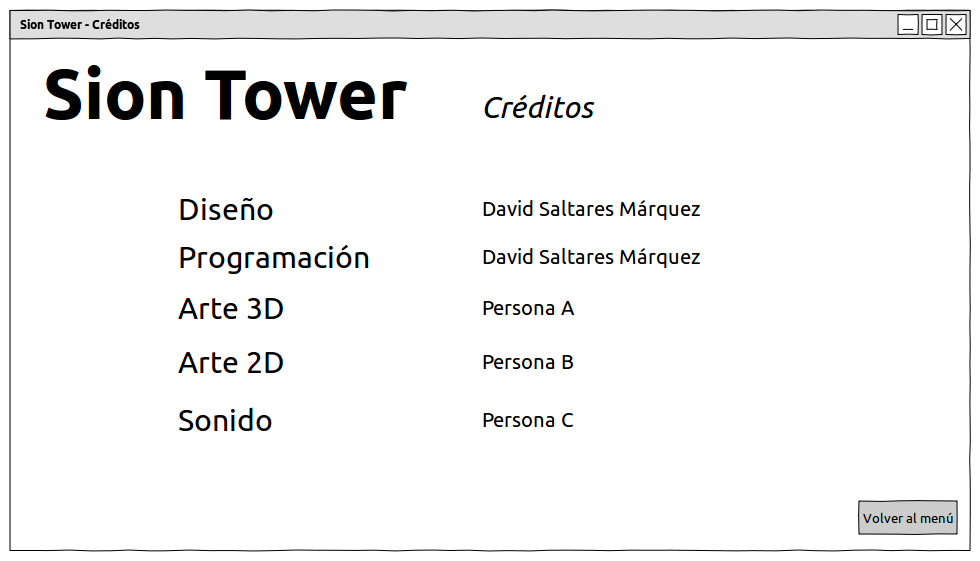
\includegraphics[width=\textwidth]{img/creditos.png} 
    \caption{Boceto de la pantalla de cŕeditos}
    \label{img:creditos}
\end{figure}

\paragraph{}
Lista y descripción de todos sus componentes.

\begin{itemize}
    \item \textbf{Panel}: texto con los componentes del equipo de desarrollo.
    \item \textbf{Botón menú}: al pulsarlo volvemos al \menu.
\end{itemize}

\clearpage

\subsection{Selección de perfil}
\label{sec:ui-perfil}

\paragraph{}
A continuación el boceto de la pantalla de \selperfil:

\begin{figure}[H]
    \centering
        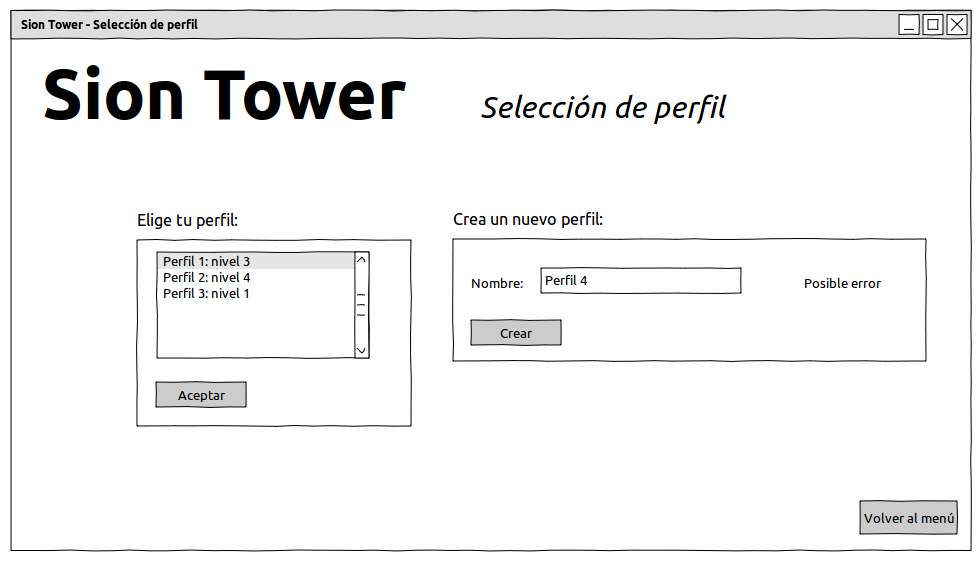
\includegraphics[width=\textwidth]{img/sel-perfil.png} 
    \caption{Boceto de la pantalla de selección de perfil}
    \label{img:sel-perfil}
\end{figure}

\paragraph{}
Lista y descripción de todos sus componentes.

\begin{itemize}
    \item \textbf{Lista de perfiles}: lista con los perfiles guardados
    hasta el momento. Se muestra el nombre del perfil y el nivel alcanzado.
    \item \textbf{Botón aceptar}: al pulsarlo se toma el perfil seleccionado
    y vamos a la pantalla de \selnivel.
    \item \textbf{Crear perfil}: etiqueta y caja de texto para introducir
    el nombre del nuevo perfil.
    \item \textbf{Botón crear}: crea un perfil nuevo con el nombre que contiene
    la caja de texto. Si el perfil existe o no se ha introducido un nombre,
    se muestra un error.
    \item \textbf{Etiqueta error}: muestra el posible mensaje de error
    al tratar de añadir un nuevo perfil.
    \item \textbf{Botón menú}: al pulsarlo volvemos al \menu.
\end{itemize}

\clearpage

\subsection{Selección de nivel}
\label{sec:ui-selnivel}

\paragraph{}
A continuación el boceto de la pantalla de \selnivel:

\begin{figure}[H]
    \centering
        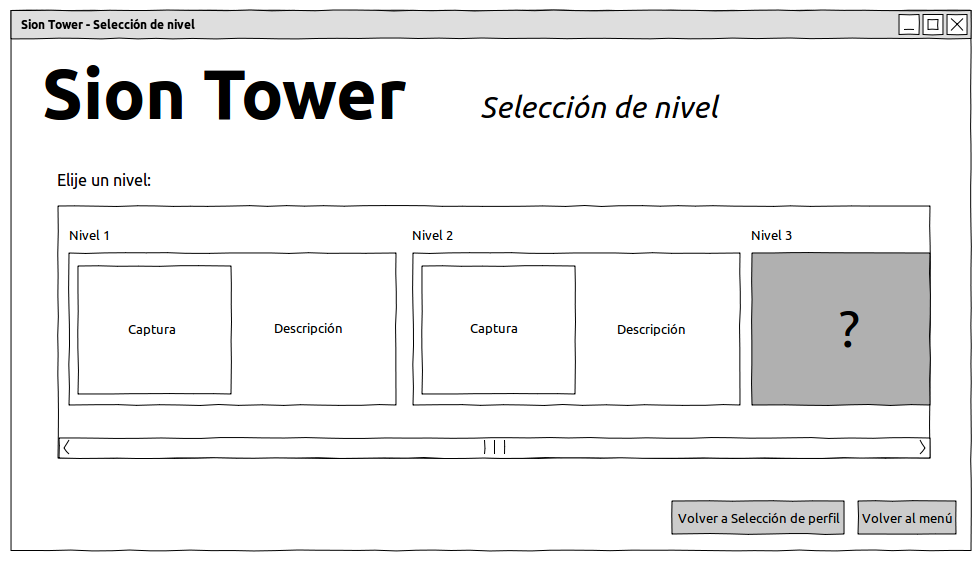
\includegraphics[width=\textwidth]{img/sel-nivel.png} 
    \caption{Boceto de la pantalla de selección de nivel}
    \label{img:sel-nivel}
\end{figure}

\paragraph{}
Lista y descripción de todos sus componentes.

\begin{itemize}
    \item \textbf{Lista de niveles}: bloque con barra de desplazamiento
    horizontal que contiene una caja por cada nivel del juego.
    \item \textbf{Bloque nivel}: cada nivel está representado por un bloque
    que contiene: el nombre del nivel, una pequeña captura y una descripción con
    los avances de la historia. Si el nivel está desbloqueado se mostrará
    con normalidad, si aún no podemos acceder aparecerá un bloque oscuro
    con una interrogación. Para seleccionar un nivel haremos click sobre su
    bloque y pasaremos a la pantalla de \selhabilidad.
    \item \textbf{Botón perfil}: al pulsarlo volvemos a la pantalla \selperfil.
    \item \textbf{Botón menú}: al pulsarlo volvemos al \menu.
\end{itemize}

\clearpage

\subsection{Selección de habilidades}
\label{sec:ui-habilidades}

\paragraph{}
A continuación el boceto de la pantalla de \selhabilidad:

\begin{figure}[H]
    \centering
        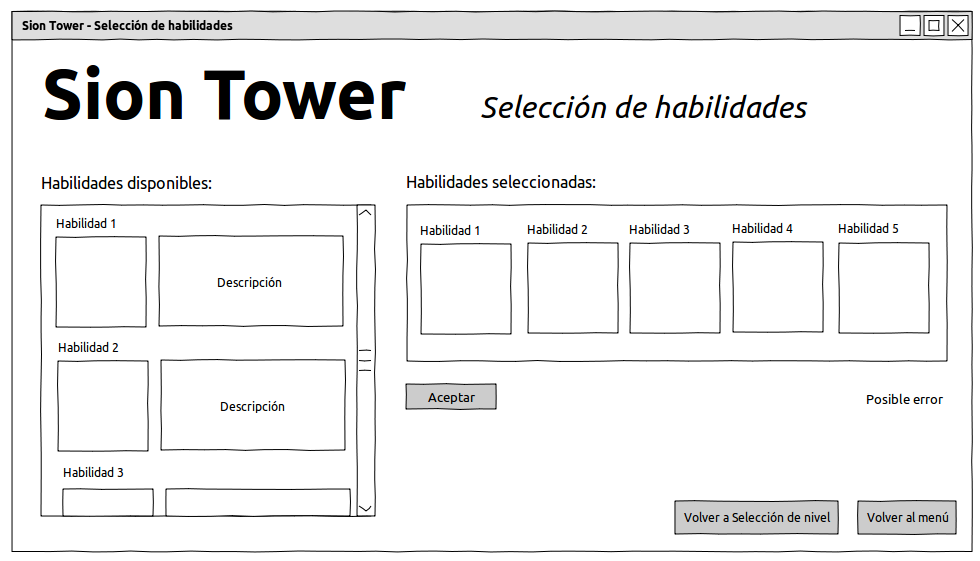
\includegraphics[width=\textwidth]{img/sel-hab.png} 
    \caption{Boceto de la pantalla de selección de habilidades}
    \label{img:sel-hab}
\end{figure}

\paragraph{}
Lista y descripción de todos sus componentes.

\begin{itemize}
    \item \textbf{Habilidades disponibles}: bloque con barra de desplazamiento
    vertical que contiene las habilidades que ha conseguido desbloquear el
    \jugador.
    \item \textbf{Bloque habilidad}: cada habilidad está formada por un bloque
    que contiene su nombre, un icono y una descripción. Al pulsar sobre una habilidad
    se añade automáticamente a la lista de habilidades seleccionadas y queda
    bloqueada en color gris. Si no quedan slots libres, se muestra el error.
    \item \textbf{Bloque seleccionadas}: contiene los slots con las habilidades
    seleccionadas hasta el momento. De cada habilidad sólo se muestra el nombre
    y el icono.
    \item \textbf{Etiqueta error}: se muestra el mensaje de error si no quedan
    slots libres.
    \item \textbf{Botón aceptar}: al pulsarlo avanzamos hacia la pantalla de \nivel.
    \item \textbf{Botón nivel}: al pulsarlo volvemos a la pantalla \selnivel.
    \item \textbf{Botón menú}: al pulsarlo volvemos al \menu.
\end{itemize}

\clearpage

\subsection{Nivel}
\label{sec:ui-nivel}

\paragraph{}
A continuación el boceto de la pantalla de \nivel:

\begin{figure}[H]
    \centering
        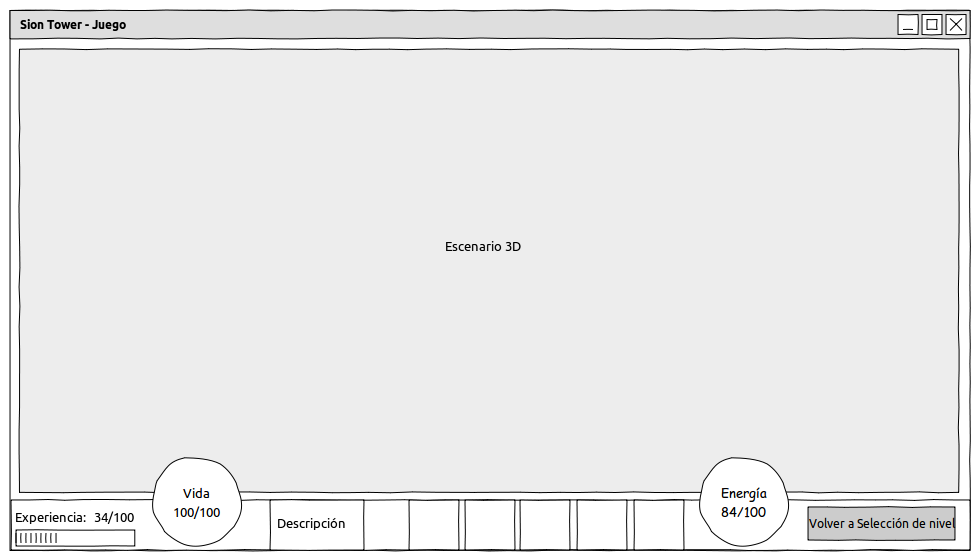
\includegraphics[width=\textwidth]{img/juego.png} 
    \caption{Boceto de la pantalla de juego}
    \label{img:juego}
\end{figure}

\paragraph{}
Lista y descripción de todos sus componentes.

\begin{itemize}
    \item \textbf{Escenario 3D}: panel de juego.
    \item \textbf{Experiencia}: etiquetas con la experiencia actual
    y la necesaria para alcanzar la siguiente habilidad. Incluye
    una barra de progreso.
    \item \textbf{Vida}: bola de contenido verde cuyo nivel varía
    según la cantidad de vida que se posee. Tiene inscrito encima el valor.
    \item \textbf{Energía}: bola de contenido azul cuyo nivel varía
    según la cantidad de energía que se posee. Tiene inscrito encima el valor.
    \item \textbf{Habilidades}: icono de las habilidades disponibles. Si
    no se tiene suficiente energía para utilizar una, ésta aparecerá
    en un tono grisáceo. Al pasar el ratón por encima de algunas, aparece
    su descripción en el recuadro de la izquierda. Para activar la habilidad,
    hacemos click sobre ella.
    \item \textbf{Descripción}: contiene la descripción de la habilidad
    activa.
    \item \textbf{Botón nivel}: al pulsarlo volvemos a la pantalla \selnivel.
\end{itemize}

\clearpage

\subsection{Fin de nivel}
\label{sec:ui-finnivel}

\paragraph{}
A continuación el boceto de la pantalla de \finnivel:

\begin{figure}[H]
    \centering
        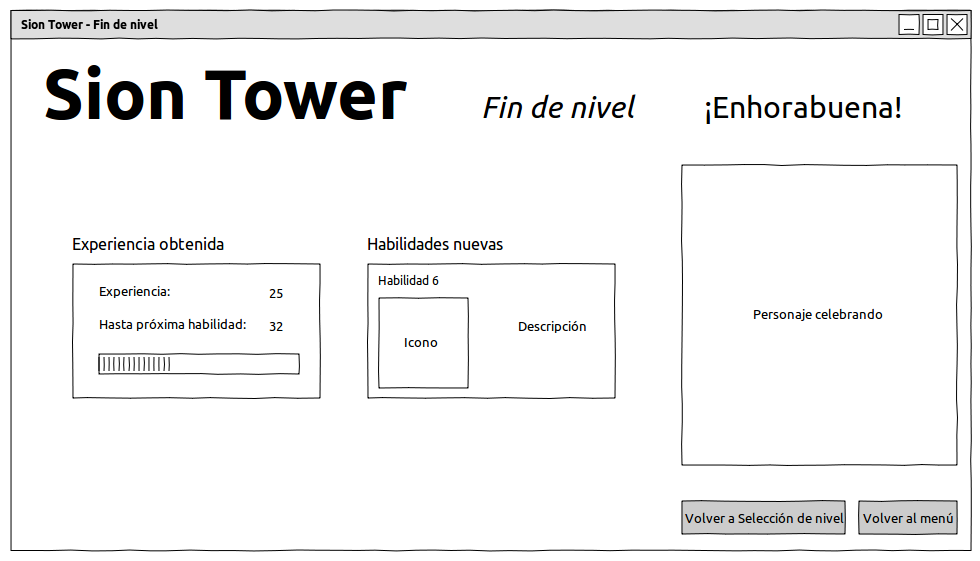
\includegraphics[width=\textwidth]{img/fin-nivel.png} 
    \caption{Boceto de la pantalla de fin de nivel}
    \label{img:fin-nivel}
\end{figure}

\paragraph{}
Lista y descripción de todos sus componentes.

\begin{itemize}
    \item \textbf{Experiencia}: bloque que muestra la experiencia obtenida
    en ese nivel y la experiencia restante para desbloquear la próxima habilidad.
    \item \textbf{Habilidad nueva}: bloque que, en el caso se haber desbloqueado
    una habilidad la mostrará (nombre, icono y descripción). 
    \item \textbf{Personaje}: protagonista en 3D celebrando la victoria.
    \item \textbf{Botón selección de nivel}: al pulsarlo volvemos a la pantalla \selnivel.
    \item \textbf{Botón menú}: al pulsarlo volvemos al \menu.
\end{itemize}
